\documentclass[12pt,a4paper]{report}
\usepackage{graphicx}
\usepackage{amsmath}
\usepackage{fancyhdr}
\usepackage{cite}
\usepackage{framed}
\usepackage{a4wide}
\usepackage{float}
\graphicspath{ {./frontpages/} }
%The below Section make chapter and its name to center of the page
\usepackage{blindtext}
\usepackage{xpatch}
\makeatletter
\xpatchcmd{\@makeschapterhead}{%
  \Huge \bfseries  #1\par\nobreak%
}{%
  \Huge \bfseries\centering #1\par\nobreak%
}{\typeout{Patched makeschapterhead}}{\typeout{patching of @makeschapterhead failed}}


\xpatchcmd{\@makechapterhead}{%
  \huge\bfseries \@chapapp\space \thechapter
}{%
  \huge\bfseries\centering \@chapapp\space \thechapter
}{\typeout{Patched @makechapterhead}}{\typeout{Patching of @makechapterhead failed}}

\makeatother
%The above Section make chapter and its name to center of the page
%\unwanted packages also included

\linespread{1.5}
%\pagestyle{fancy}
%\fancyhead{}
%\header and footer section
%\renewcommand\headrulewidth{0.1pt}
%\fancyhead[L]{\footnotesize \leftmark}
%\fancyhead[R]{\footnotesize \thepage}
%\renewcommand\headrulewidth{0pt}
%\fancyfoot[R]{\small College of Engineering, Kidangoor}
%\renewcommand\footrulewidth{0.1pt}
%\fancyfoot[C]{2019 - 2020}
%\fancyfoot[L]{\small Name of the project}




\begin{document}
\begin{center}
{\Large \textbf{EXTREME ULTRAVIOLET LITHOGRAPHY}}\\
\vspace{2cm}
A SEMINAR REPORT\\
\vspace{0.5cm}
Submitted by \\
\vspace{1cm}
\textbf{ABHIJITH S}\\
\vspace{0.2cm}
\textbf{KGR18EC001}\\
\vspace{0.2cm} to\\


 the A P J Abdul Kalam Technological University \\
in partial fulfillment of the requirements for the award 
of the Degree \\
of\\
Bachelor of Technology \\
in\\
Electronics and Communication Engineering
\end{center}


\begin{center}

\vspace{1.2cm}


\includegraphics[scale=0.3]{ceklogo.jpg}

DEPARTMENT OF ELECTRONICS \& COMMUNICATION ENGINEERING\\

COLLEGE OF ENGINEERING KIDANGOOR\\

JANUARY 2022\\
\end{center}

\thispagestyle{empty}
\newpage
%\Declaration in this page.
\begin{center}
\textbf{DECLARATION}\\
\end{center}
I hereby declare that the seminar report \textbf{“Extreme Ultraviolet Lithography”} , 
submitted for partial fulfillment of the requirements for the award of degree of 
Bachelor of Technology in Electronics and Communication Engineering of the APJ 
Abdul Kalam Technological University, Kerala is a bonafide work done by me
under supervision of Mr. Joby James. This submission represents my ideas in
 my own words and where ideas or words of others have been included, I 
 have adequately and accurately cited and referenced the original sources. 
 I also declare that I have adhered to ethics of academic honesty and 
 integrity and have not misrepresented or fabricated any data or idea 
 or fact or source in my submission. I understand that any violation 
 of the above will be a cause for disciplinary action by the Institute 
 and/or the University and can also evoke penal action from the sources 
 which have thus not been properly cited or from whom proper permission 
 has not been obtained. This report has not been previously formed the 
 basis for the award of any degree, diploma or similar title of any other 
 University.

\noindent \begin{minipage}{0.45\linewidth}
\begin{flushleft}
\vspace{1 cm}
                         
Kidangoor \\
Date\\

\end{flushleft} 
\end{minipage}
\hfill
\begin{minipage}{0.45\linewidth}
\begin{flushright}                                      
\vspace{1cm}
                         
Abhijith S\\


\end{flushright} 
\end{minipage}

\thispagestyle{empty}

\newpage
\begin{center}

%\vspace{1.5cm}

\textbf{Department of Electronics and Communication Engineering}

\textbf{COLLEGE OF ENGINEERING KIDANGOOR}


\textbf{2018-2022}
\end{center}
\begin{center}
% \includegraphics[scale=0.25]{CEK-emblem.jpg}

\end{center}
\vspace{0.2cm}
\begin{center}
 \textbf{CERTIFICATE}
\end{center}

This is to certify that the report entitled \textbf{ \large EXTREME ULTRAVIOLET LITHOGRAPHY} 
submitted by \textbf{ABHIJITH S}, to the APJ Abdul Kalam Technological University in 
partial fulfillment of the Bachelor of Technology degree in Electronics 
and Communication Engineering is a bonafide record of the seminar work 
carried out by him/her under our guidance and supervision.
\vspace{3cm}

\noindent \begin{minipage}{0.45\linewidth}
\begin{flushleft}
\vspace{3cm}
                         
\textbf{Seminar Coordinator} \\
\vspace{0.8cm}
Mr. Joby James \\
\footnotesize{Assistant Professor\\
Electronics and Communication\\
College of Engineering Kidangoor}\\

\end{flushleft} 
\end{minipage}
\hfill
\begin{minipage}{0.35\linewidth}
\begin{flushleft}                                      
\vspace{3cm}
                         
\textbf{Head of the Department} \\
\vspace{.8cm}
Dr. Rajeesh J\\
\footnotesize{Professor\\
Electronics and Communication\\
College of Engineering Kidangoor}\\


\end{flushleft} 
\end{minipage}
\thispagestyle{empty}

\newpage
\chapter*{\centering \large ACKNOWLEDGEMENT\markboth{Acknowledgements}{Acknowledgements}}

This is the most satisfying, yet most difficult 
part of the seminar to present gratifying words 
because most often they fail to convey the real 
influence, others have had on one’s work. I would 
like to take this opportunity to extend my sincere
 gratitude to Dr.RAJEESH J, Head of Electronics and 
 Communication Department for extending every facility 
 to complete my seminar work successfully.I would like 
 to express my sincere indebtedness to ASST.PROFESSOR 
 JOBY JAMES, Department of Electronics and Communication,
 for his valuable guidance,wholehearted co-operation 
 and duly approving the topic as staff in charge. 
 I also thank all my teachers and  friends for their 
 sincere guidance and cooperation. Above all I thank 
 The Almighty for his abundant blessings without
which this seminar would not have been success.



\begin{flushright}
\textbf{Abhijith S}
\end{flushright}
\thispagestyle{empty}


% Please remove and edit percentage(%) Symbol, if you want this 
% Acknowledgement page in your report. As per ktu guideline, 
% this page is not necessary. 
\begin{abstract}

%\pagenumbering{roman}
As we all know, an integrated circuit or chip is one of the 
biggest innovations of the 20th 
century it launched many of the technological innovations 
and revolutions created in silicon valley.
at big tech conferences, chip manufacturers will announce  
they've hit impossibly small new mile stone, like 22nm 
then 14 nm and 10 nm designs. 
that means they've found a way to shrink the size and 
increase the number
of features on a chip, which ultimately improves the 
overall processing power. 
this is what's been driving the semiconductor industry, 
which is also called Moore's law.
Unfortunately, Moore's Law is starting to fail: 
transistors have become so small 
that simple physics began to block the process
Moore's law has been predicted to be dying for a long 
time and yet it never is.
because each
generation engineers knows it's their expectation to 
keep working on it, going at a certain pace.
EUVL is such an NGL that keeps Moore's law alive


Extreme ultraviolet lithography (also known as EUV or EUVL) 
is  a lithography (mainly chip printing/making aka "fabricating") 
technology using  a range of extreme ultraviolet (EUV) wavelengths, 
roughly spanning a 2\% FWHM bandwidth about 13.5 nm. While EUV 
technology is available for  mass production, only 53 machines 
worldwide capable of  producing wafers using the technique 
were delivered during 2018 and 2019,  while 201 immersion 
lithography systems were delivered during the same  period. 
Extreme ultraviolet lithography (EUVL) technology and 
infrastructure  development has made excellent progress 
over the past several years, and  tool suppliers are 
delivering alpha tools to customers. Potential successors 
to optical projection lithography are being aggressively 
developed. These are known as "Next-Generation Lithographies" 
(NGL's). EUV lithography (EUVL) 
is one of the leading NGL technologies; others include x-ray 
lithography, ion beam projection lithography, and electron-beam 
projection lithography. Using extreme-ultraviolet (EUV) light 
to carve transistors in silicon wafers will lead to 
microprocessors that are up to 100 times faster than 
today's most powerful chips, and to memory chips 
with similar increases in storage capacity.  
Significant efforts are also needed to achieve the 
resolution, line width  roughness, and photo speed 
requirements for EUV photoresists. Cost of  ownership 
and extendibility to future nodes are key factors in 
determining the  outlook for the manufacturing insertion 
of EUVL. Since wafer throughput is a  critical cost 
factor, source power, resist sensitivity, and system 
design all need  to be carefully considered. However, 
if the technical and business challenges  can be met, 
then EUVL will be the likely technology of choice for 
semiconductor  manufacturing at the 32, 22, 16 and 11 
nm half-pitch nodes
\end{abstract}
\pagenumbering{roman}
\tableofcontents %This command used for index.
\listoffigures




    

\chapter{INTRODUCTION}
\pagenumbering{arabic}
After three decades of development, a new generation of 
lithography machines has now been shipped to large 
computer chip makers. It uses extreme ultraviolet (EUV) 
light at a wavelength of 13.5 nm to make silicon 
features down to a few nanometers in size on the 
memory chips and processors of tomorrow.with more than 
100,000 components, such an EUV 
lithography system is one of the most complex 
machines ever built. It is pumped by the most 
powerful laser system ever made in serial production. 
In total, it weighs 180 tons and consumes more than 
1 MW electrical power. It costs \$120 million

Extreme ultraviolet (sometimes also called XUV) denotes 
soft x-rays with wavelengths between 124 and 10 nm or
 photon energies between 10 eV and 124 eV. 
 The sun produces EUV; humans create it through 
 synchrotrons, or from plasma.
Up until now, chip makers have used ultraviolet light to 
project complex patterns onto
 silicon wafers coated with photoresist. In a process 
 analogous to the development of the old paper photos, 
 these patterns are developed and become conducting or 
 isolating structures within one layer. This process is 
 repeated until the complex systems forming an 
 integrated circuit such as a microprocessor are 
 complete.The development of such lithographic systems is 
driven by economy: Ever more computing power 
and storage capacity is needed while costs and 
power consumption must be lowered. 
This development can be described in a simple rule, 
well-known as Moore’s law

\section{Moore's Law}
Moore's law is an observation and projection of a 
historical trend. Rather than a law 
of physics, Moore's law is an expectation it's 
not like a natural law or something. An expectation 
that we innovate at a pace of roughly doubling 
the density of transistors on a IC every two years.
All these allow us to 
offer better products, allow us to offer cheaper 
products with the same capability and that in 
turn drives the demand for the overall industry. 
that means that we've got to be able to cram in, 
more and more
functionality per square millimeter on a chip. all 
the design and everything have to be smaller in dimensions.


\begin{figure}
  \centering
  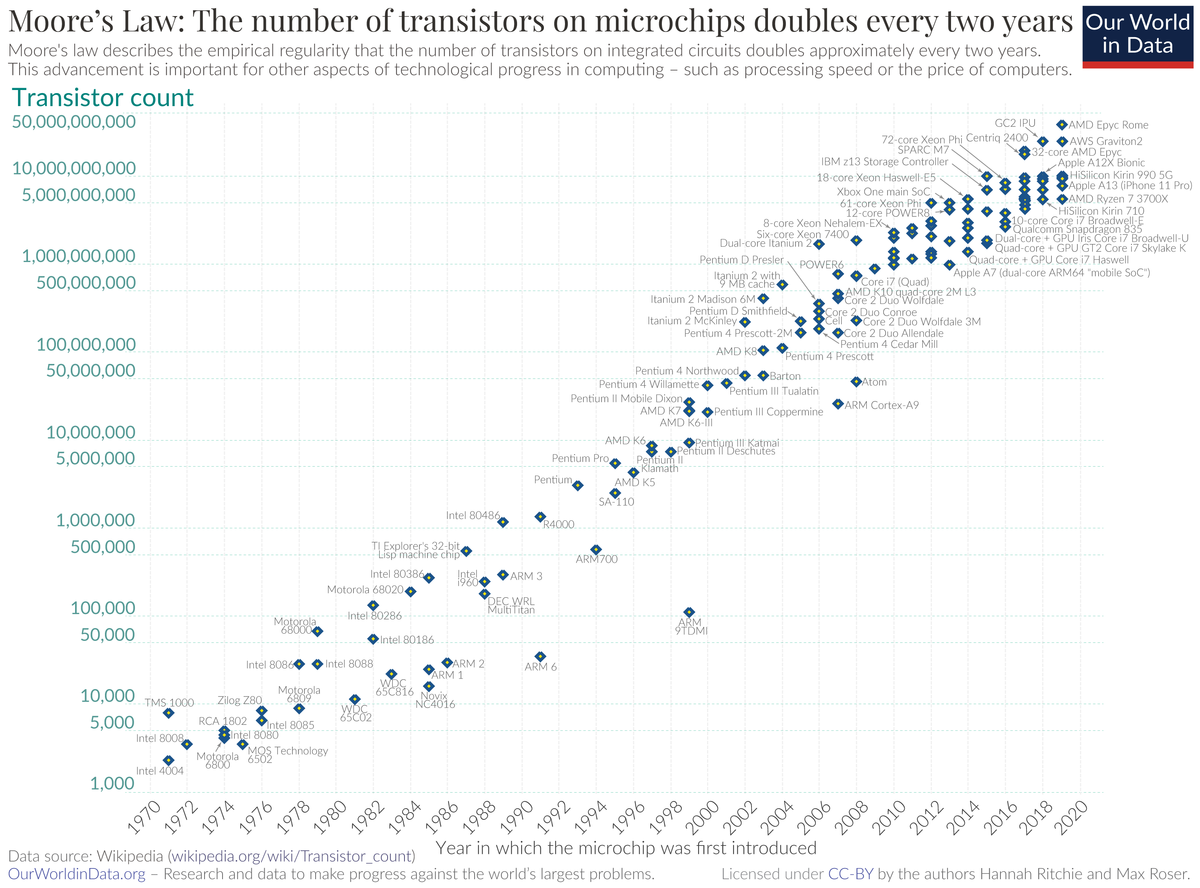
\includegraphics[scale=0.3]{Moore's_Law_Transistor_Count.png}
  \caption{Moore's Law Transistor Count}
  \label{arch}
  \end{figure}

\section{Photolithography}
Photolithography, also called optical lithography or UV lithography, 
is a process used in 
microfabrication to pattern parts on a thin film or the bulk of 
a substrate (also called a wafer). 
It uses light to transfer a geometric pattern from a photomask 
(also called an optical mask) to 
a photosensitive (that is, light-sensitive) chemical photoresist 
on the substrate. A series of 
chemical treatments then either etches the exposure pattern into 
the material or enables deposition 
of a new material in the desired pattern upon the material 
underneath the photoresist

This method can create extremely small patterns, down to a few 
tens of nanometers in size. 
It provides precise control of the shape and size of the objects 
it creates and can create 
patterns over an entire surface cost-effectively. It's main 
disadvantages are that it requires 
a flat substrate to start with, it is not very effective at 
creating shapes that are not flat, 
and it can require extremely clean operating conditions. 
Photolithography is commonly used to produce computer chips. 
When producing computer chips, 
the substrate material is a resist covered wafer of silicon. 
This process allows hundreds of 
chips to be simultaneously built on a single silicon wafer.





\section{Basic Concept}
Major limitation in the lithography process comes from 
the laws of optics. 
German physicist Ernst Abbe found that the resolution 
of a microscope d is 
(roughly) limited to the 
wavelength $\lambda$ of the light used in illumination:

$$d =\lambda/(nsin(\alpha))$$


where n is the refractive index of the medium between the 
lens and the object and 
$\lambda$ is the half-angle of the objective's cone of 
light. For lithography, substituting
numerical aperture (NA) for $$nsin(\alpha)$$ and adding 
a factor k to the formula 
(because lithographic resolution can be strongly tweaked 
with illumination tricks),
the minimum feasible structure, or critical dimension 
(CD), is:

$$CD = {k}{\lambda}/NA$$


This formula, which governs all lithographic imaging processes, makes 
obvious why the wavelength is such a crucial parameter. As a result, 
engineers have been looking for light sources with ever-shorter 
wavelengths to produce ever-smaller features. Beginning with UV
 mercury-vapor lamps, they moved to excimer lasers with a wavelength of 193 nm. 



\chapter{EUVL}
\section{Introduction to EUVL}

Optical projection lithography is the technology used to
print the intricate patterns that define integrated circuits
onto semiconductor wafers. Typically, a pattern on a
mask is imaged, with a reduction of 4:1, by a highly
accurate camera onto a silicon wafer coated with
photoresist. Continued improvements in optical
projection lithography have enabled the printing of ever
finer features, the smallest feature size decreasing by
about 30\% every two years. This, in turn, has allowed
the integrated circuit industry to produce ever more
powerful and cost-effective semiconductor devices. On
average, the number of transistors in a state-of-the-art
integrated circuit has doubled every 18 months.
Currently, the most advanced lithographic tools used in
high-volume manufacture employ deep-ultraviolet (DUV)
radiation with a wavelength of 248 nm to print features
that have line widths as small as 200 nm. It is believed
that new DUV tools, presently in advanced development,
that employ radiation that has a wavelength of 193 nm,
will enable optical lithography to print features as small
as 100 nm, but only with very great difficulty for highvolume manufacture. Over the next several years it will
be necessary for the semiconductor industry to identify a
new lithographic technology that will carry it into the
future, eventually enabling the printing of lines as small
as 30 nm. Potential successors to optical projection
lithography are being aggressively developed. These are
known as “Next-Generation Lithographies” (NGL's).
EUV lithography (EUVL) is one of the leading NGL
technologies; others include X-Ray lithography, ionbeam projection lithography, and electron-beam
projection lithography.
In many respects, EUVL may be viewed as a natural
extension of optical projection lithography since it uses
short wavelength radiation (light) to carry out projection
imaging. In spite of this similarity, there are major
differences between the two technologies. Most of these
differences occur because the properties of materials in
the EUV portion of the electromagnetic spectrum are
very different from those in the visible and UV
wavelength ranges. The purpose of this paper is to
explain what EUVL is and why it is of interest, to
describe the current status of its development, and to
provide the reader with an understanding of the
challenges that must be overcome if EUVL is to fulfill its
promise in high-volume manufacture.

EUVL technology is an advanced technology with a 
light source of 13.5 nm, which is extremely short 
wavelength and can be applied for beyond the 10 
nm node. EUVL enables the use of only one mask 
exposure instead of multiexposure. However, there 
are still three issues to be solved before this 
technique can be applied in mass production: a 
light power source, resists, and mask infrastructure. 
Among these issues, to make such a lithography tool, 
economical production capacity and producing a 
stable light source are the most difficult issues 
to be solved. For a wafer-per-hour (WPH) up to 125 
in the 12-inch production line, a light source 
power of 200 W is needed and EUVL has to satisfy 
this requirement.
The development of resist material is one of 
the critical technical issues of EUVL. This 
material is necessary to have the excellent 
characteristics: high resolution, high sensitivity 
as well as low line-edge roughness (LER) and low 
outgassing simultaneously.
When EUVL continues to move toward mass 
production manufacturing, the availability 
of a defect-free reflective photomask is also 
one of the critical challenges which needs to 
be considered. EUV's photomasks work in 
reflective mode. To produce these masks would 
introduce new materials and surfaces, which 
might cause high particle adhesion on the surface 
of masks, creating a cleaning issue. 
Therefore, a special pellicle is designed to 
protect the mask from particles adhesion when 
the EUV scanner is in use. However, an EUV mask 
with a pellicle has still some remaining issues 
to be solved. These issues are also addressed: 
the stress of the protective film module may 
cause an overlay shift; it may also prevent 
the film from light absorbing, and the mask 
inspection can be limited to photochemical light, 
which reduces the valuable EUV power.
In addition to EUV technology, very extremely 
short wavelength techniques such as using the 
X-ray lithography (XRL) with 1 nm wavelength 
 and deep X-ray lithography (DXRL) with 0.1 nm 
 wavelength are under development and they 
 belong to next-generation lithography (NGL), 
 which may provide a solution for technology 
 node beyond 5 nm in future.

\section{Why EUV ?}

In order to keep pace with the demand for the printing of
ever smaller features, lithography tool manufacturers
have found it necessary to gradually reduce the
wavelength of the light used for imaging and to design
imaging systems with ever larger numerical apertures.
The reasons for these changes can be understood from
the following equations that describe two of the most
fundamental characteristics of an imaging system:
resolution (RES) and depth of focus (DOF). These
equations are usually expressed as

$$RES = {k_1}{\lambda}/NA$$

where l is the wavelength of the radiation used to carry
out the imaging, and NA is the numerical aperture of the
imaging system (or camera). These equations show that
better resolution can be achieved by reducing l and
increasing NA. The penalty for doing this, however, is
that the DOF is decreased. Until recently, the DOF used
in manufacturing exceeded 0.5 mm, which provided for
sufficient process control.
The case k1 = k2 = ½ corresponds to the usual definition
of diffraction-limited imaging. In practice, however, the
acceptable values for k1 and k2 are determined
experimentally and are those values which yield the
desired control of critical dimensions (CD’s) within a
tolerable process window. Camera performance has a
major impact on determining these values; other factors
that have nothing to do with the camera also play a role.
Such factors include the contrast of the resist being used
and the characteristics of any etching processes used.
Historically, values for k1 and k2 greater than 0.6 have
been used comfortably in high-volume manufacture.
Recently, however, it has been necessary to extend
imaging technologies to ever better resolution by using
smaller values for k1 and k2 and by accepting the need for
tighter process control. This scenario is schematically
diagrammed in Figure 1, where the values for k1 and
DOF associated with lithography using light at 248 nm
and 193 nm to print past, present, and future CD’s
ranging from 350 nm to 100 nm are shown. The
“Comfort Zone for Manufacture” corresponds to the
region for which k1 > 0.6 and DOF > 0.5 mm. Also
shown are the k1 and DOF values currently associated
with the EUVL printing of 100 nm features, which will
be explained later. As shown in the figure, in the very
near future it will be necessary to utilize k1 values that
are considerably less than 0.5. Problems associated with
small k1 values include a large iso/dense bias (different
conditions needed for the proper printing of isolated and
dense features), poor CD control, nonlinear printing
(different conditions needed for the proper printing of
large and small features), and magnification of mask CD
errors. Figure 1 also shows that the DOF values
associated with future lithography will be uncomfortably
small. Of course, resolution enhancement techniques
such as phase-shift masks, modified illumination
schemes, and optical proximity correction can be used to
enhance resolution while increasing the effective DOF.
However, these techniques are not generally applicable to
all feature geometries and are difficult to implement in
manufacturing. The degree to which these techniques
can be employed in manufacturing will determine how
far optical lithography can be extended before an NGL is
needed.
% Lithography with 193 nanometer light has been 
% pushed further than many would 
% have thought possible, but it has come at a cost: 
% the industry has had to reach 
% deep into a bag of tricks to continue shrinking 
% chip features. Chipmakers will be 
% able to continue making smaller, faster and 
% more powerful chips while keeping 
% costs in check.


% \begin{figure}
% \centering
% \includegraphics[scale=0.5]{Substrate.jpg}
% \caption{Elements of Biological cells and components of a typical IoT device.}{Ref- [2]}
% \label{sub}
% \end{figure}

\section{Working}

working: 
EUVL is a significant departure from the deep 
ultraviolet lithography standard. 
Attached to the EUV scanner, the source consists 
of a droplet generator, collector and a vacuum chamber. 
In EUV, the process takes place in a vacuum 
environment, because nearly everything absorbs 
EUV light.
{All optical elements, including the photomask,
 must use defect-free molybdenum/silicon (Mo/Si) 
 multilayers (consisting of 40 Mo/Si bilayers) that 
act to reflect light by means of interlayer 
interference; any one of these mirrors absorb
 around 30\% 
of the incident light.
}

The source of the light is a tiny little droplet of tin.
 they're smaller than 
the diameter of a human hair in which we fire 
across the vessel and then we intercept those 
with a pulsed laser 
beam of very high power and have to hit with 
an accuracy of just a few microns
The droplets are 25 microns in diameter and 
are falling at a rate of 50,000 times a second


In the vessel, there is a camera. A droplet 
passes a certain position in the chamber. 
Then, the camera tells the seed laser in the 
sub-fab to fire a laser pulse into the main 
vacuum chamber. This is called the pre-pulse

Then comes the really hard part. The pre-pulse 
laser hits the spherical tin droplet and turns 
it into a pancake-like shape. Then the laser 
unit fires again, representing the main pulse. 
The main pulse hits the pancake-like tin droplet
 and vaporizes it.


At that point, the tin vapor becomes plasma. 
The plasma, in turn, emits EUV light at 13.5nm 
wavelengths

The goal is to hit a droplet with precision
This determines how much of the laser power 
gets turned into EUV light, 
which is referred to as conversion efficiency

this {video illustrates the process}
There's a collector mirror that collects that light
and sends it into the scanner. then there are 
four mirrors that essentially shape that light 
into a slit that
bounces off the reticle.
The light bounces off the collector and travels 
through an intermediate focus unit into the scanner
then you will see a reticle stage doing this, 
and a wafer stage doing this {Video}

and what's  happening is step and scan. which 
basically means we continue to reproduce that 
particular pattern
over and over again

EUV light is propelled into the scanner. In the 
scanner, the light bounces off a complex scheme 
of 10 surfaces or multi-layer mirrors. First, 
the light goes through a programmable illuminator. 
This forms 
a pupil shape to illuminate the right amount of 
light for the EUV mask.

Then, EUV light hits the mask, which is also 
reflective. It bounces off six multi-layer 
mirrors in the
projection optics. Finally, the light hits 
the wafer at an angle of 6%.

EUV photomasks work by reflecting light, which is 
achieved by using multiple alternating layers of 
molybdenum and silicon. 
This is in contrast to conventional photomasks 
which work by blocking light using a single 
chromium layer on a quartz substrate. An EUV mask 
consists of 40 alternating silicon and molybdenum 
layers;
[7] this multilayer acts to reflect the extreme 
ultraviolet light through Bragg diffraction; 
the reflectance is a strong function of incident 
angle and wavelength, with longer wavelengths 
reflecting more near normal incidence and shorter 
wavelengths reflecting more away from normal incidence. 
The pattern is defined in a tantalum-based 
absorbing layer over the multilayer.
 The multilayer 
may be protected by a thin ruthenium layer.


Current EUVL systems contain at least two 
condenser multilayer mirrors, six projection multilayer 
mirrors and a multilayer object (mask). Since 
the mirrors absorb 96\% of the EUV light, the ideal 
EUV source needs to be much brighter than its 
predecessors. EUV source development has focused on 
plasmas generated by laser or discharge pulses. 
The mirror responsible for collecting the light is 
directly exposed to the plasma and is vulnerable 
to damage from high-energy ions and other 
debris[19] such as tin droplets, which require 
the costly collector mirror to be replaced every year.

Very precise  extremely flat micro-mirrors to 
focus the light onto the silicon wafer to 
produce even finer feature widths.



% \begin{figure}[ht]
% \centering
% \includegraphics[scale=0.5]{molec commun.jpg}
% \caption{Examples of Molecular Communication} {Ref- [2]}
% \label{commun}
% \end{figure}


\section{EUVL mask}

Photoresists are a critical part of lithography. Resists are 
light-sensitive materials. 
They form patterns on a surface when exposed to light. For EUV, 
they are critical.
The basic requirements for EUVL resist are sensitivity, 
resolution, Line Width Roughness 
(LWR) or Line Edge Roughness (LER), outgassing, a pattern 
cross-sectional aspect ratio 
and profile, etch resistance, defect density, and 
reproducibility. Among them, 
it is a critical challenge to meet the requirements 
simultaneously on resolution, 
LWR, and sensitivity (RLS). EUVL uses Chemically Amplified 
Resist (CAR) due to 
the advantages of high sensitivity and resolution, but its 
LWR is relatively high, 
which becomes a significant issue. For the 22 nm feature, 
LWR should be 
controlled below 2 nm, which is about half of the current 
best available values

\chapter{SECURITY IN IoBNT}
The advent of skin implanted bio-electronics and the IoBNT 
paradigm will not only open up a plethora of novel biomedical
 applications but also its wireless connection capability will
  enable the adversaries to utilize it malevolently. Connecting
   the intra-body biological environment with the cyber domain
    through bio-electronic devices will provide the attackers 
    with an apparent opportunity to devise new terrorist 
    mechanisms to harm the patient remotely. Maliciously 
    accessing the human body through the internet to steal 
    personal information or to create new types of diseases 
    by malevolent programming of bio-electronic devices and 
    intra-body nanonetworks is termed as bio-cyber terrorism. 
    Bio-cyber terrorism can take advantage of wirelessly 
    accessing the human body to launch fatal and 
    life-threatening attacks from a remote site. 
    Therefore security features have to be embedded either
     in a separate component of the bio-electronic device, 
     which may enlarge the size of the device or might be
      infeasible in some applications. Another possibility is
       to delegate security services to external devices in 
       close proximity with sophisticated resources as compared
        to bioelectronics devices. Nonetheless, the bio-electronic
         device must execute a lightweight authentication mechanism
         at least once to establish a secure connection with external
          devices. Bio-electronic devices will also be linked to a
          gateway device (such as a smartphone) to send and receive 
          information from the healthcare practitioner. Because of 
          the technological differences, this section discusses the 
          security needs for nanonetworks and bio-cyber interfaces 
          separately. The security goals, regardless of the underlying 
          technological variations, remain the same. The STRIDE threat 
          approach can be used to model security threats against IoBNT. 
          STRIDE is the acronym for Spoofing, Tampering, Repudiation, 
          and Information Disclosure, Denial of Service and Elevation 
          of privilege. These six categories present a broad classification 
          of threats and can be further divided into other related threats.
          Each threat category is related to a security goal: Spoofing-Authentication, 
          Tampering-Integrity, Repudiation, Non-Repudiation, Information Disclosur, 
          Confidentiality, Denial of Service- Availability, and Elevation of 
          privileges-Authorization.

\textbf{Integrity (I)}: Integrity ensures that the message 
exchanged between legitimate entities is not tampered or 
modified by unauthorized entities.

\textbf{Non- Repudiation (NR)}: In the traditional networking 
paradigm, all the communication transactions are logged to 
track the network anomalies and gain the attacker’s profile 
in case the attacker tries to misuse his/her privileges. 
Non-repudiation can be violated if the attacker gets access 
to the logs and delete the records to remove traces.

\textbf{Confidentiality (C)}: Confidentiality ensures that the 
attacker should not learn the content of the message exchanged 
between the sender and receiver. The data must only be accessible
 to authorized personnel upon authentication through some mechanism priory.

\textbf{Availability (A)}: This goal ensures that the services
 and communication of the device is always available on request.

\textbf{Authorization (Auth)}: Authorization property ensures 
that only those entities can execute a specific operation that
 has privileges to order it. Authorization requires that an 
 entity must have been authenticated previously through the 
 regular login (ID, password) procedure to establish the identification.

\chapter{ATTACKS IN IoBNT}
Identification of attacks and threats is also important for 
network security. The attacks can be performed by two types 
of attackers; Internal attackers and External attackers.

Internal attackers are part of the system and have access to 
credentials and other information required to communicate with 
other system entities.

External attackers in the scenario of nano communication can be
 divided into two types: Local and remote attackers. Local 
 attackers are located in the vicinity of attacked nanosystem.
 Attacks like eavesdropping and spoofing can be performed by 
 these attackers. Remote attackers have to become local attackers before launching the attack.
The types of attacks launched by these attackers are classified into four groups:

\textbf{Disclosure}: These types of threats include access to 
the system by unauthorized users. In the case of nano-networks,
 these types of attacks are complex to launch when using mechanical
 or molecular communication. However electromagnetic and acoustical
  communication opens the door for the attackers as the covered 
  area is relatively large.

\textbf{Deception}: Attackers can falsify or manipulate data in
 this type of attack. Injecting false information in the network
  can challenge system reliability. Integrity checks can be 
  performed to limit these attacks. However computational protection schemes

\textbf{Disruption}: The availability and reliability can be 
stalled by this kind of attack. Given in the context of
 nano-networks the attacker can modify the parameters such
  as temperature and pH level to disrupt communication.

\textbf{Usurpation}: Unauthorized entities can control system 
services or entities, beyond just disrupting the system. This 
attack can enable attackers to cause malfunctions or even take 
over the entire system.

\chapter{APPLICATIONS OF IoBNT}
\section{Intra-body sensing and actuation}
Intra-body sensing and actuation, where
Bio-NanoThings inside the human body
would collaboratively collect health-related
information, transmit it to an external
healthcare provider through the Internet,
and execute commands from the same provider such as synthesis and release of drugs.
\section{ Intra-body connectivity control}
 Intra-body connectivity control, where BioNanoThings would repair
  or prevent failures in the communications between our internal 
  organs, such as those based on the
endocrine and the nervous systems, which
are at the basis of many diseases.
\section{Environmental control and cleaning}
Environmental control and cleaning, where
Bio-NanoThings deployed in the environment, such as a natural ecosystem, would
check for toxic and pollutant agents, and
collaboratively transform these agents
through bioremediation, e.g. bacteria
employed to clean oil spills.
\section{PANACEA}
PANACEA (a solution or remedy for all difficulties or diseases 
in Latin) is presented as a solution for an end-to-end design 
towards realizing the IoBNT for the first time in the literature. 
The architecture of PANACEA is tailored to focus on diagnosis and 
therapy of infectious diseases. In PANACEA, to detect the 
communication within the cells of the body to deduce infection 
level, a submillimeter implantable bio-electronic device, a 
Bio-NanoThing, is proposed. BNT can transmit the detected 
infection data remotely to a wearable hub/gateway outside of the body. 
The hub can use mobile devices and the backbone network such as 
Internet or cellular systems to reach the healthcare providers 
who can remotely control the BNTs. Hence, PANACEA provides a system, 
where sensing, actuation and computing processes are tightly coupled 
to provide a reliable and responsive disease detection and infection 
recovery system. system will continuously monitor the tissues at risk 
of serious infection to detect it earlier than conventional methods
 which requires culturing the bacteria in a laboratory to increase 
 its quantity to detectable levels, which typically takes 48-72 hours.
 While alternative molecular methods such as enzyme-linked immunosorbent 
 assay (ELISA) and polymerase chain reaction (PCR) provide higher 
 sensitivity and specificity within a shorter assay time, they 
 require complex instrumentation and skilled operators limiting 
 their use to clinical laboratories. As such, these methods are 
 not suitable for continuous in vivo monitoring for early detection 
 of infections. The proposed system eavesdropping on the quorum 
 sensing (QS) communication among infectious bacteria in the tissue 
 by distributed BNTs which host electronic devices and highly 
 miniaturized bio-sensors. QS is a method of communication where 
 bacteria coordinate their behavior by exchange of molecules. 
 By listening in to QS via BNTs, the spatio-temporal distribution
 of abnormally growing bacteria in tissue can be obtained to 
 detect an infection even before the patient shows symptoms. 
 QS signals are transformed into electrical signals measured 
 and converted into raw data relayed through the coil/antenna
  to the wearable hub, which may come in the form of a patch,
   bandage, or smartwatch. The wearable hub forwards the raw 
   data via access networks such as wi-fi or cellular systems
    to the Internet where it is processed and delivered to 
    interested parties such as healthcare institutes and 
    emergency services, and send an actuator information if required.
    Besides the early detection of infections, we can use IoBNT 
    framework to help us with the mitigation of infections by 
    incorporating active and passive drug delivery systems. 
    For passive drug delivery, external devices can be configured
     to release the pre-programmed drug recipe or send a message 
     to patients to take personalized medicine. For active drug 
     delivery, a mechanism can be incorporated in the implantable 
     devices to release drugs.
% \begin{figure}[ht]
% \centering
% % \includegraphics[scale=0.5]{Panacea.jpg}
% \caption{Overview of PANACEA}{Ref- [3]}.
% \label{panacea}
% \end{figure}



\chapter{CONCLUSION}
IoBNT is an emerging research domain that holds significant
promises in various healthcare applications. These applications
 range from early symptom detection to remote diagnosis
to treatments of patients (e.g., via targeted drug delivery),
and so on. The design and integration of device components
are dependent on individual IoBNT deployment requirements
and settings (e.g., in sensing applications, relevant sensors
must be integrated to sense individual biochemical substances
like pH, sodium, and calcium). However, there are a number of 
challenges.The field of security in to IoBNT technologies is not
yet mature, generating opportunities for attackers, even
non-sophisticated attacks can have a significant impact on
both IoBNT technologies and users’ safety. Apart from software
 and hardware security mechanisms, there is a need for user’s 
 training and awareness for wide adoption of these novel technologies. 
 One of the future plans is to build and implement systems that can
  detect and mitigate security attacks affecting the theragnostics
   process in real time.

\begin{thebibliography}{99}
\bibitem{ref1} Sidra Zafar; Mohsin Nazir; Taimur Bakhshi; 
Hasan Ali Khattak; Sarmadullah Khan; Muhammad Bilal; 
Kim-Kwang Raymond Choo; Kyung-Sup Kwak; Aneeqa Sabah, 
“A Systematic Review of Bio-Cyber Interface Technologies 
and Security Issues for Internet of Bio-Nano Things,“ 
IEEE Access, no.38, pp. 21016092, June.2021.

\bibitem{ref2}I. F. Akyildiz, M. Pierobon, S. Balasubramaniam, 
and Y. Koucheryavy,‘‘The Internet of bio-nano things,’’ IEEE
 Commun. Mag., vol. 53, no. 3,pp. 32–40, Mar. 2015.

\bibitem{ref2}Ian F. Akyildiz , Maysam Ghovanloo ,Ulkuhan Guler3, Tevhide 
Ozkaya-Ahmadov,A.Fatih Sarioglu, And Bige D. Unluturk,” PANACEA: 
An Internet of Bio-NanoThings Application for Early Detection and 
Mitigation of Infectious Diseases”IEEE Access, no.10,pp. 3012139, Aug.2020.

\end{thebibliography}
\end{document}